\section{Meta-Analysis of Claimed Emergent Abilities}

Analyzing the GPT family is possible because the models are publicly queryable.
However, other model families claimed to exhibit emergent abilities are not publicly queryable, nor are their generated outputs publicly available, meaning we are limited to analyzing the published results themselves \cite{ganguli2022predictability, wei2022emergent, wei2022bigbench}.
Our alternative explanation makes two predictions.
\begin{enumerate}
    \item At the ``population level" of Task-Metric-Model Family triplets, emergent abilities should appear predominantly on specific \textit{metrics}, not \textit{task-model family} pairs, and specifically with nonlinear and/or discontinuous metrics.
    \item On individual Task-Metric-Model Family triplets that display an emergent ability, changing the metric to a linear and/or continuous metric should remove the emergent ability.
\end{enumerate}

% First, whether model families display emergent capabilities should be metric dependent, with sharp metrics being more likely to produce emergent abilities.
% Second, on task-metric-model family triplets that display emergence, considering less sharp metrics should display little-to-no emergence.
To test these predictions, we used to claimed emergent abilities on BIG-Bench \cite{srivastava2022beyond, wei2022emergent} due to the benchmark being pertinent and publicly available.

\paragraph{Prediction: Emergent Abilities Should Appear with Metrics, not Task-Model Families}

If emergent abilities are real, one should expect task-model family pairs to show emergence for all reasonable metrics. However, if our alternative explanation is correct, we should expect emergent abilities to appear only under certain metrics. To test this, we analyzed on which metrics emergent abilities appear. To determine whether a task-metric-model family triplet exhibits a possible emergent ability, we used a metric from previous work \cite{srivastava2022beyond}. Letting $y_i \in \mathbb{R}$ denote model performance at model scales $x_i \in \mathbb{R}$, sorted such that $x_i < x_{i+1}$, the emergence score is:
%
\begin{equation}
    \text{Emergence Score}\Big(\Big\{ (x_n, y_n) \Big\}_{n=1}^N \Big) \quad \defeq \quad \frac{\text{sign}(\arg \max_i y_i - \arg \min_i y_i)(\max_i y_i - \min_i y_i)}{\sqrt{\text{Median}(\{ (y_i - y_{i-1})^2 \}_i)}}
\end{equation}


\begin{figure}
    \centering
    \begin{minipage}[c]{0.7\textwidth}
     \centering
        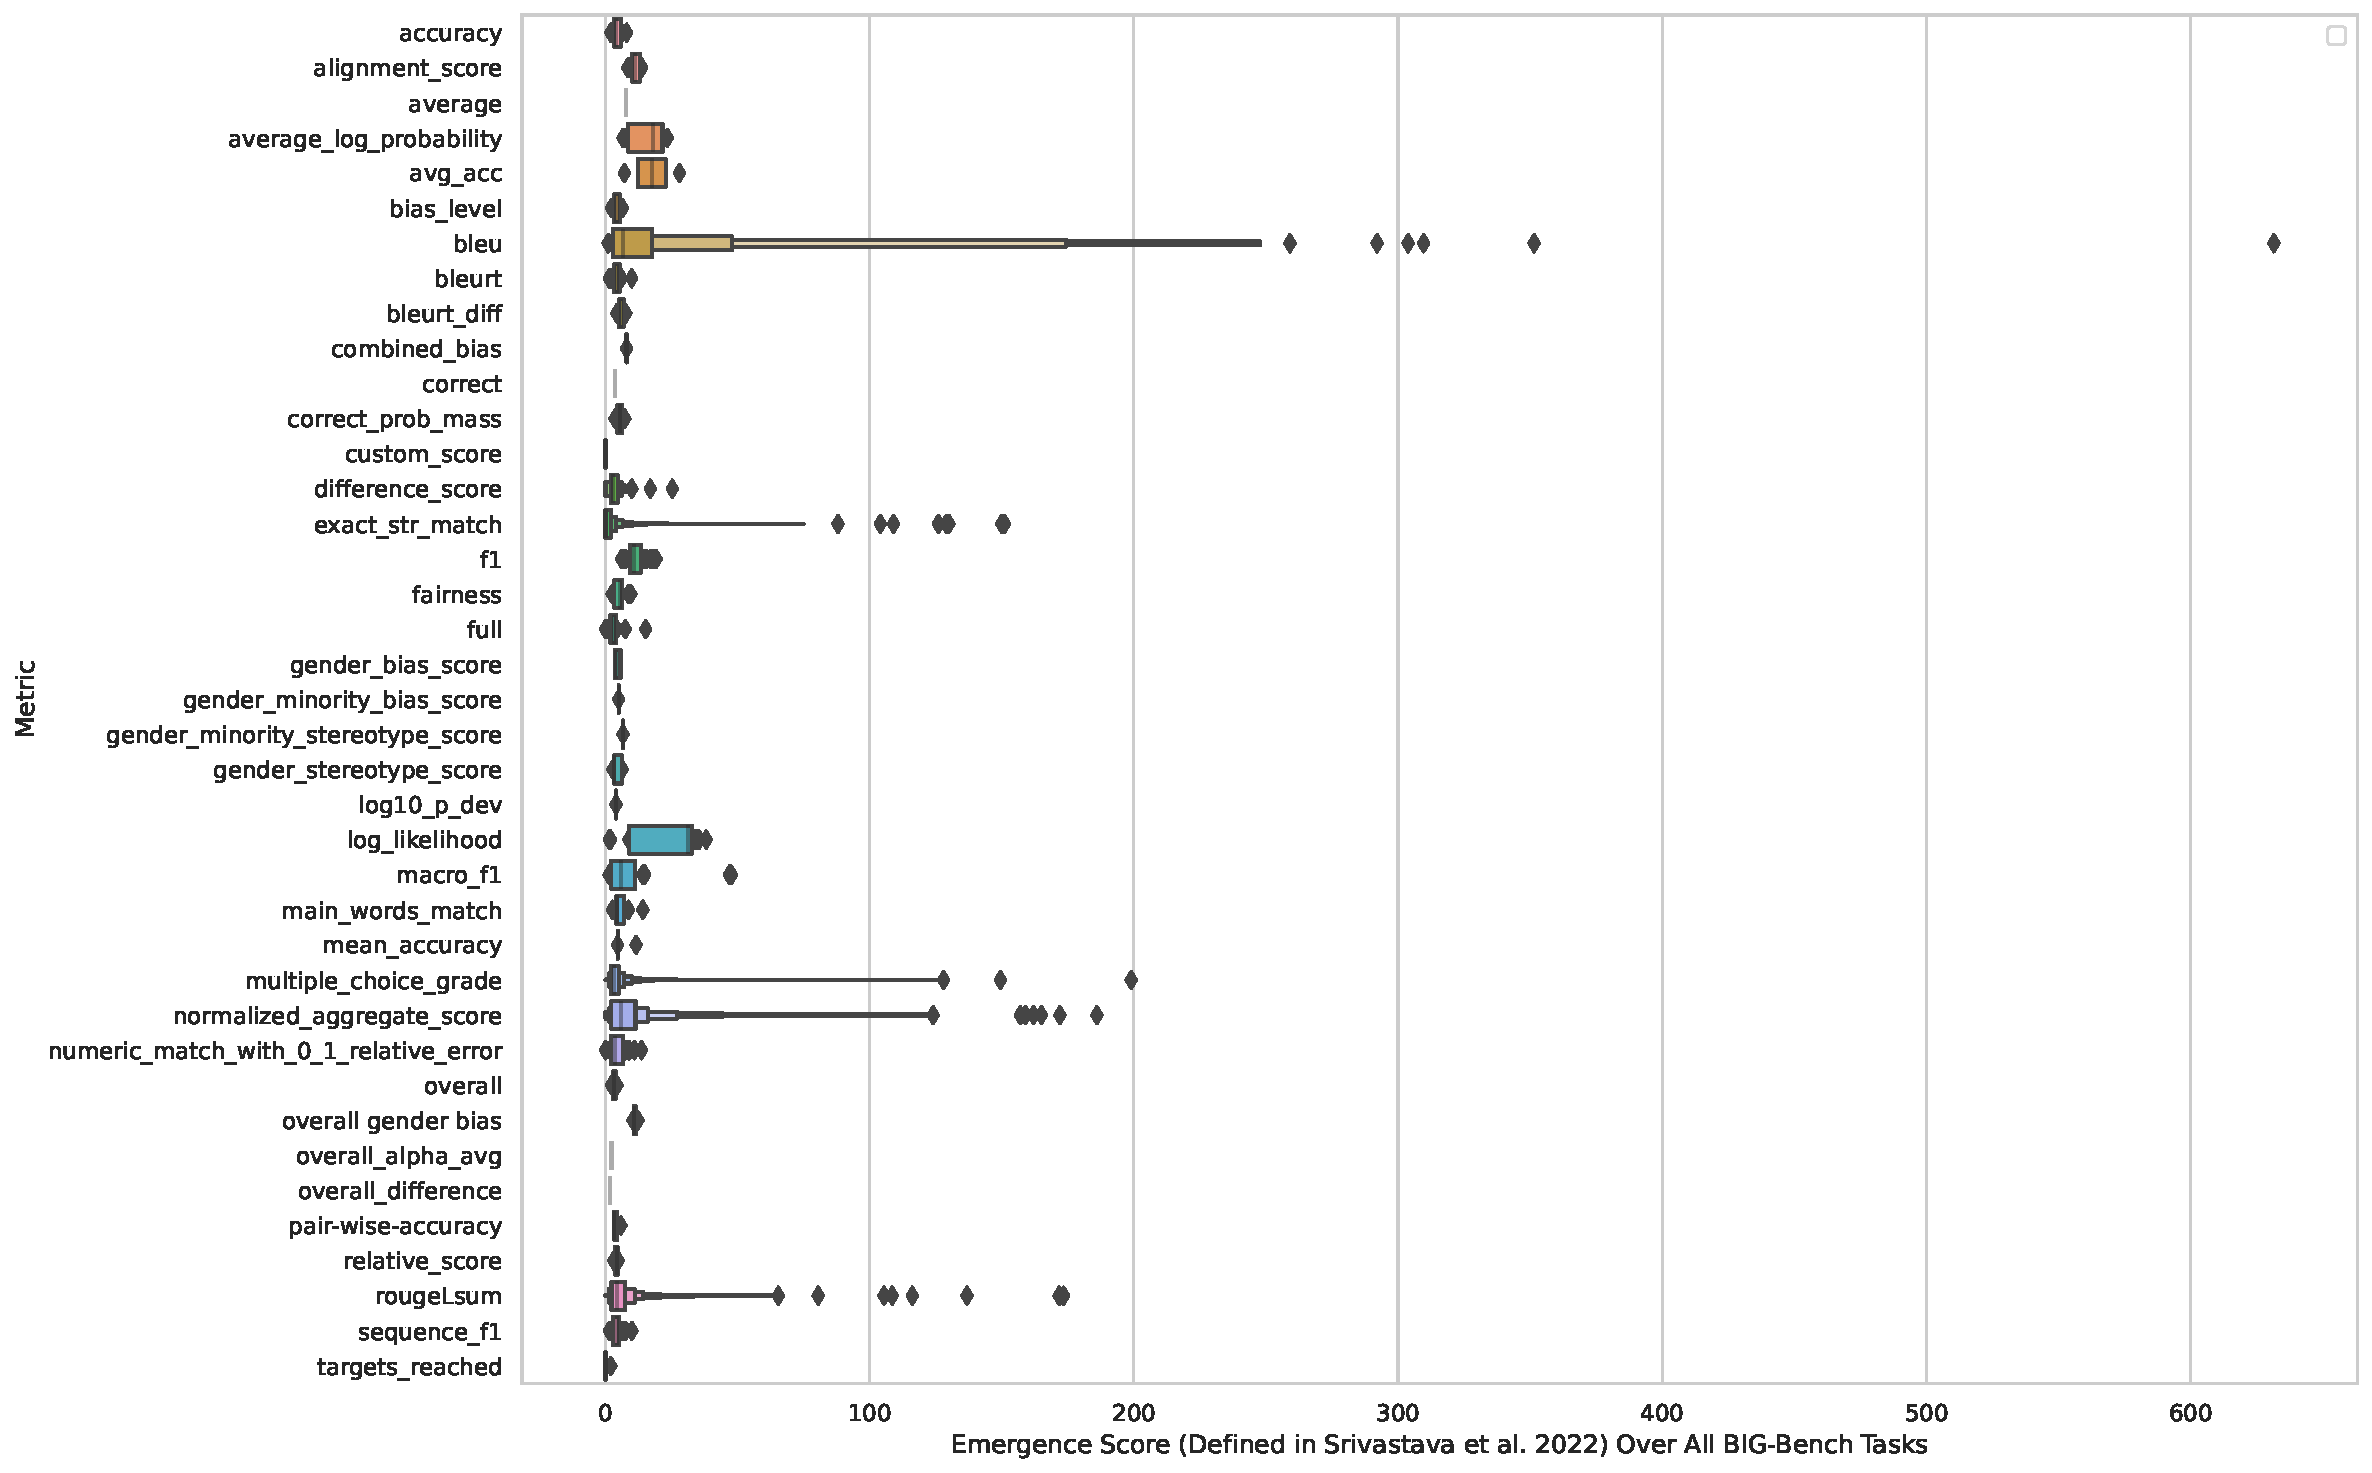
\includegraphics[width=0.95\textwidth]{figures/big_bench_emergent_tasks/big_bench_breakthrough_scores_by_metric.pdf}%
     \end{minipage}%
     \begin{minipage}[c]{0.3\textwidth}
     \centering
        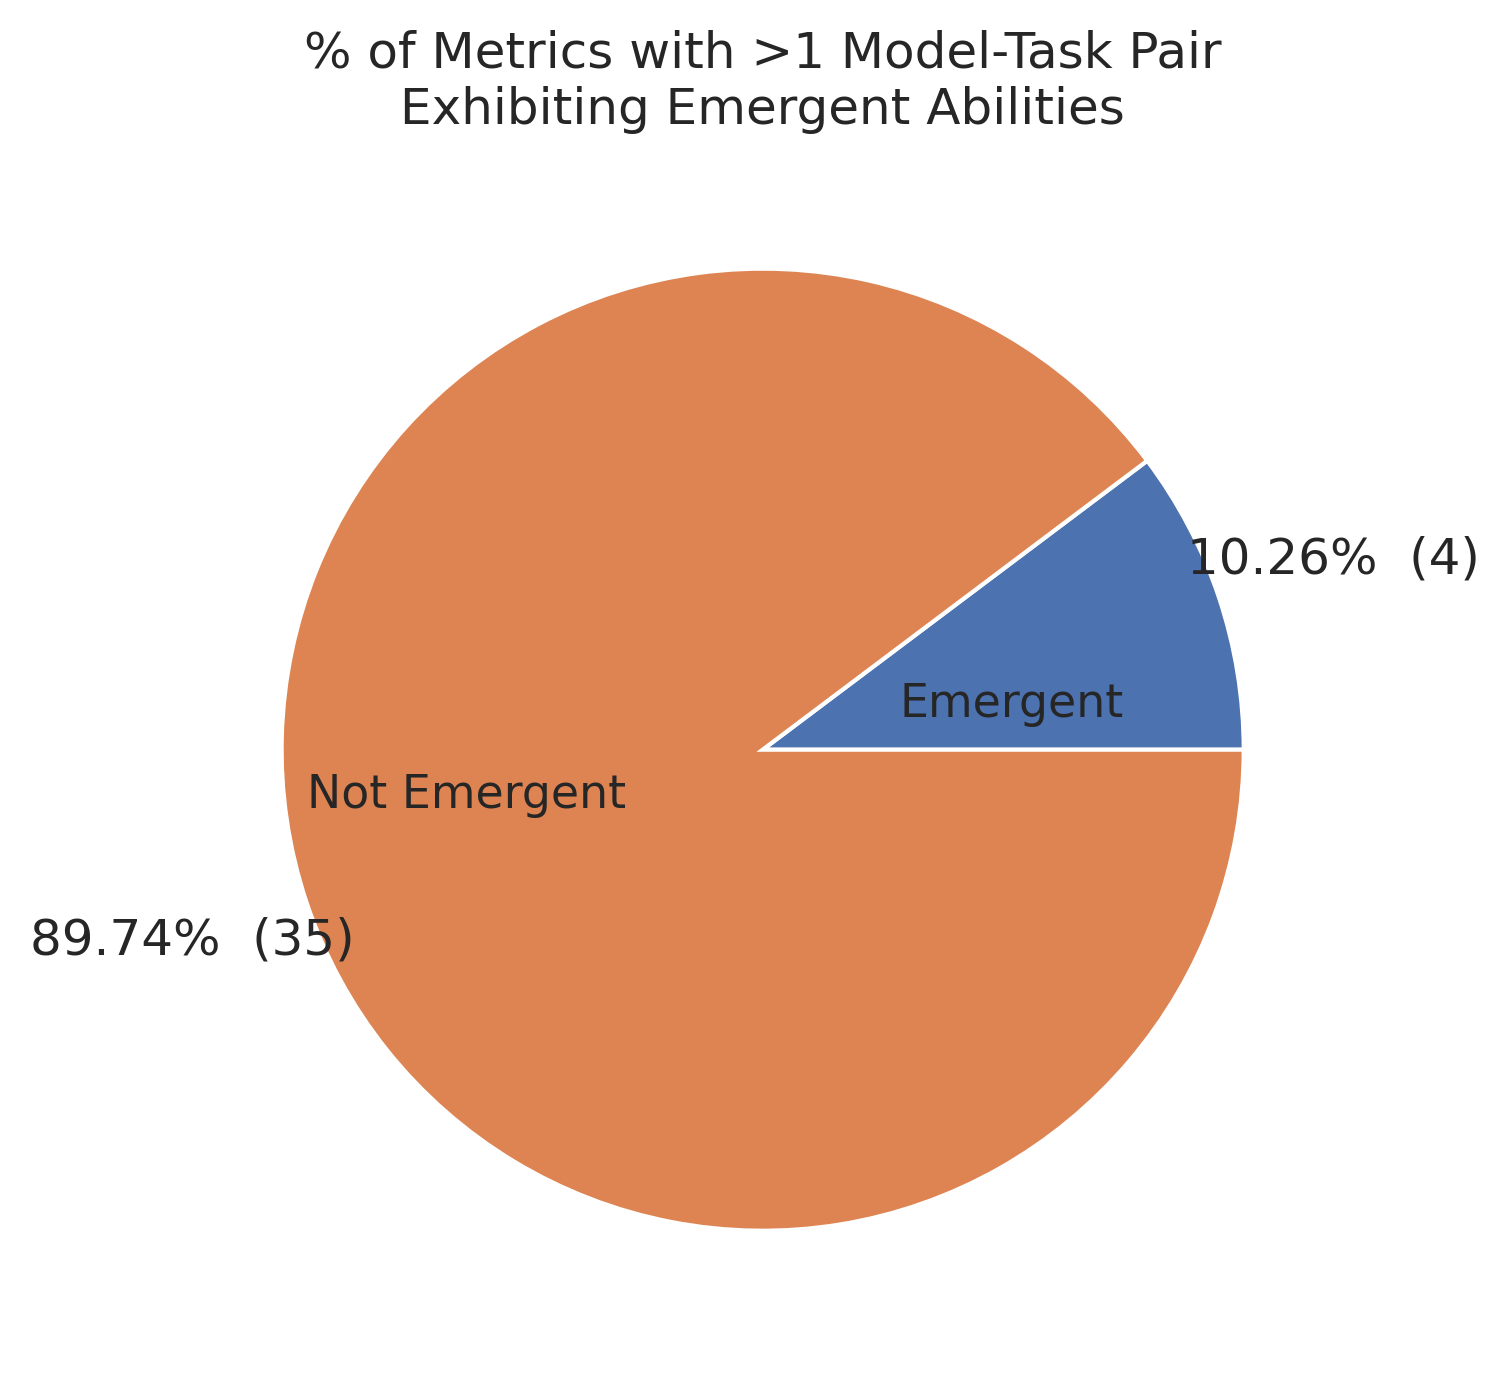
\includegraphics[width=0.85\textwidth]{figures/big_bench_emergent_tasks/emergence_percent_pie.png}
        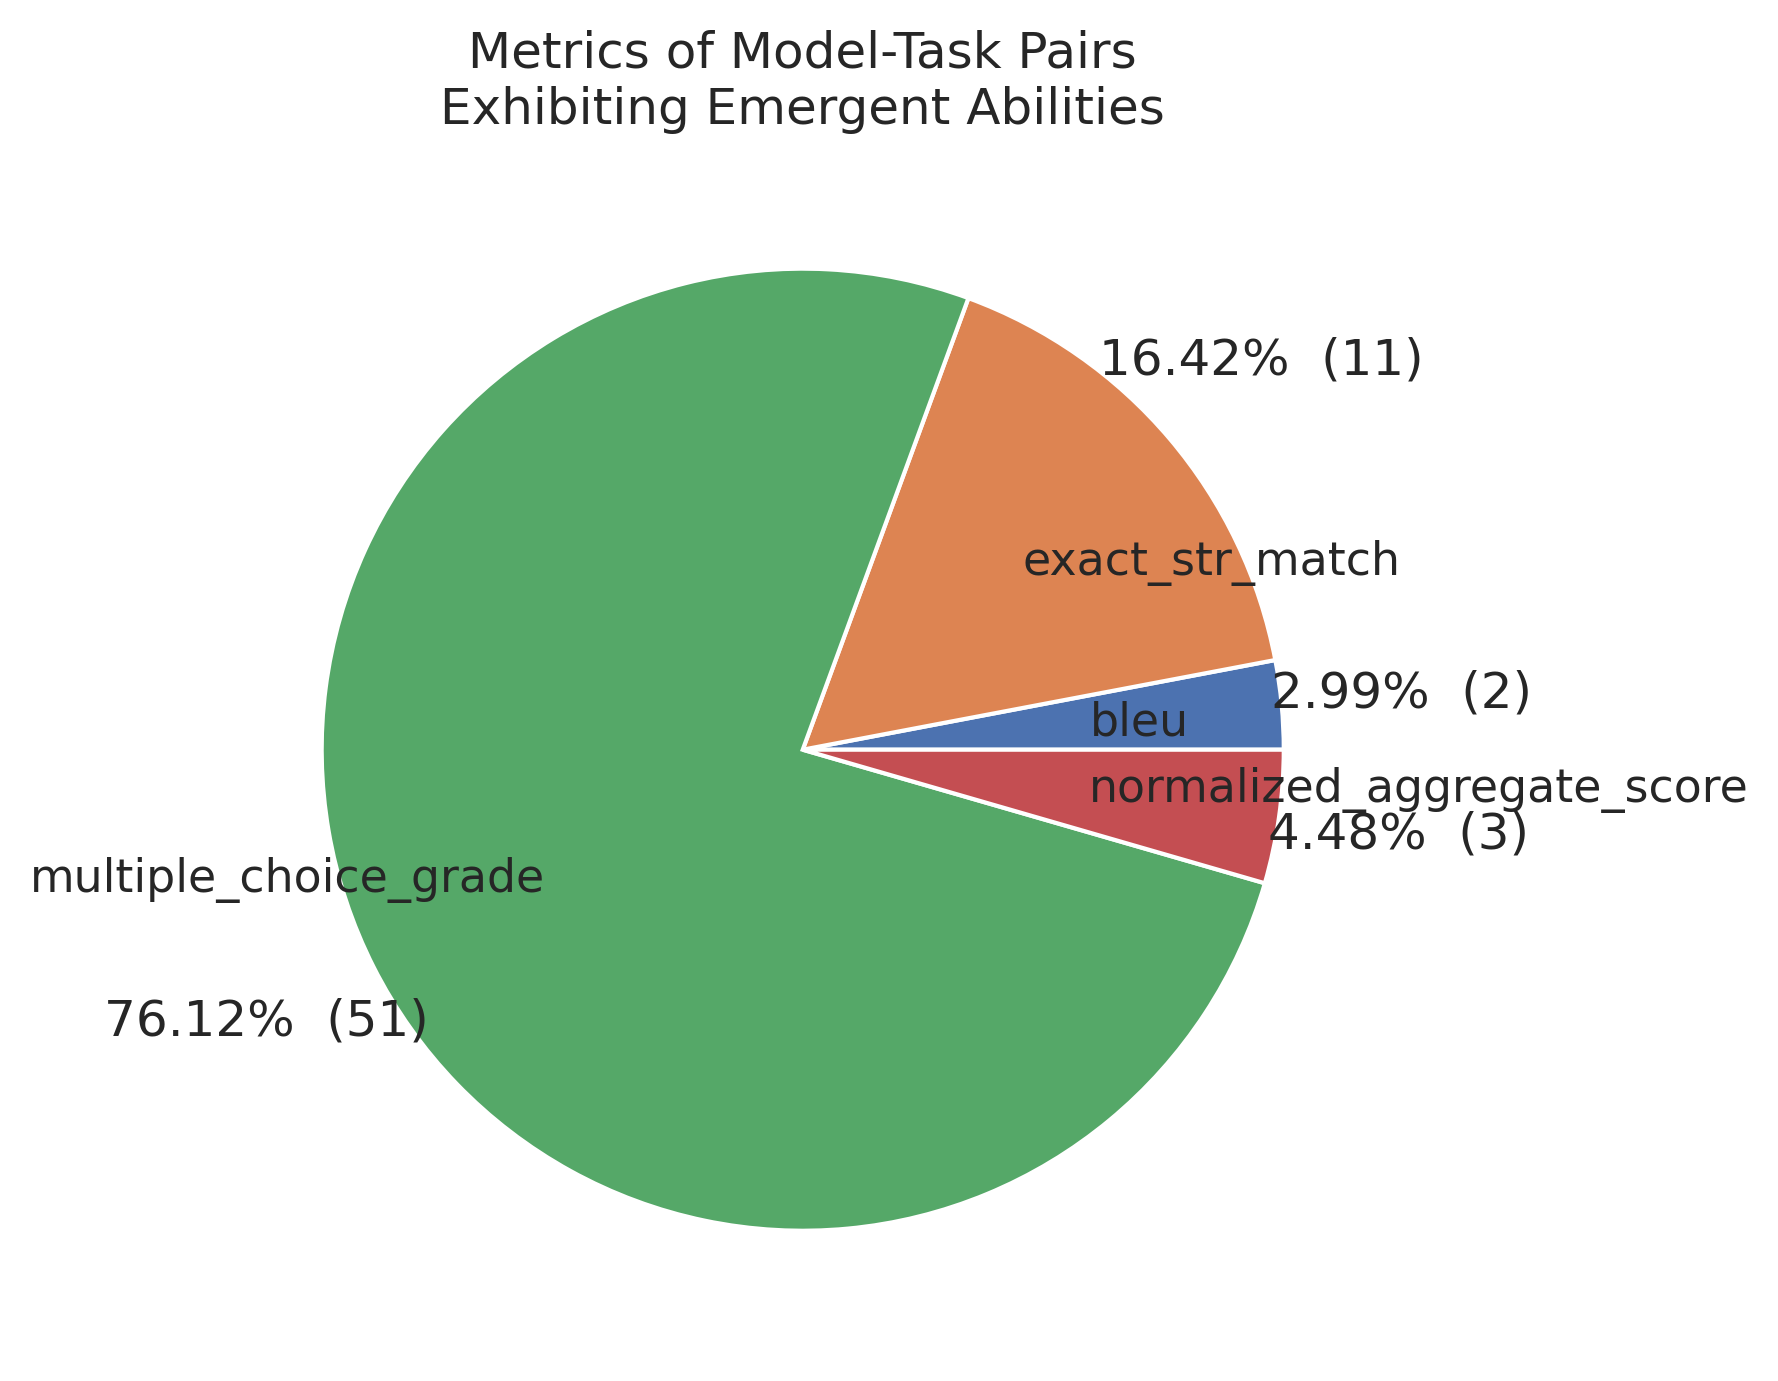
\includegraphics[width=0.95\textwidth]{figures/big_bench_emergent_tasks/metric_given_emergent_pie.png}
     \end{minipage}
    \caption{\textbf{Emergent abilities appear only for specific metrics, not task-model families.} (A) \textit{Possible} emergent abilities appear with \textit{at most} 5 out of 39 BIG-Bench metrics. (B) Hand-annotated data by \cite{wei2022bigbench} reveals emergent abilities appear only under 4 preferred metrics. (C) $>92\%$ of emergent abilities appear under one of two metrics: Multiple Choice Grade and Exact String Match.}
    \label{fig:big_bench_breakthrough_scores_by_metric}
\end{figure}

We found that most metrics used in BIG-Bench have \textit{zero} task-model family pairs that exhibit emergent abilities: of the 39 preferred metrics in BIG-Bench, at most 5 display emergence (Fig. \ref{fig:big_bench_breakthrough_scores_by_metric}A). Many of the 5 are nonlinear and/or discontinuous, e.g., Exact String Match, Multiple Choice Grade, ROUGE-L-Sum (App. \ref{app:metric_scaling:rougeLsum}). Notably, because BIG-Bench often scores models on tasks using multiple metrics, the \textit{lack} of emergent abilities under other metrics suggests that emergent abilities do not appear when model outputs are scored using other metrics.

Because emergence score only \textit{suggests} emergence, we also analyzed hand-annotated task-metric-model family triplets \cite{wei2022bigbench}, which revealed emergent abilities appear with $4 / 39$ metrics (Fig. \ref{fig:big_bench_breakthrough_scores_by_metric}B), and 2 metrics account for $>92\%$ of claimed emergent abilities (Fig. \ref{fig:big_bench_breakthrough_scores_by_metric}C): Multiple Choice Grade and Exact String Match. Multiple Choice Grade is discontinuous, and Exact String Match is nonlinear.


 \begin{figure}
    \centering
    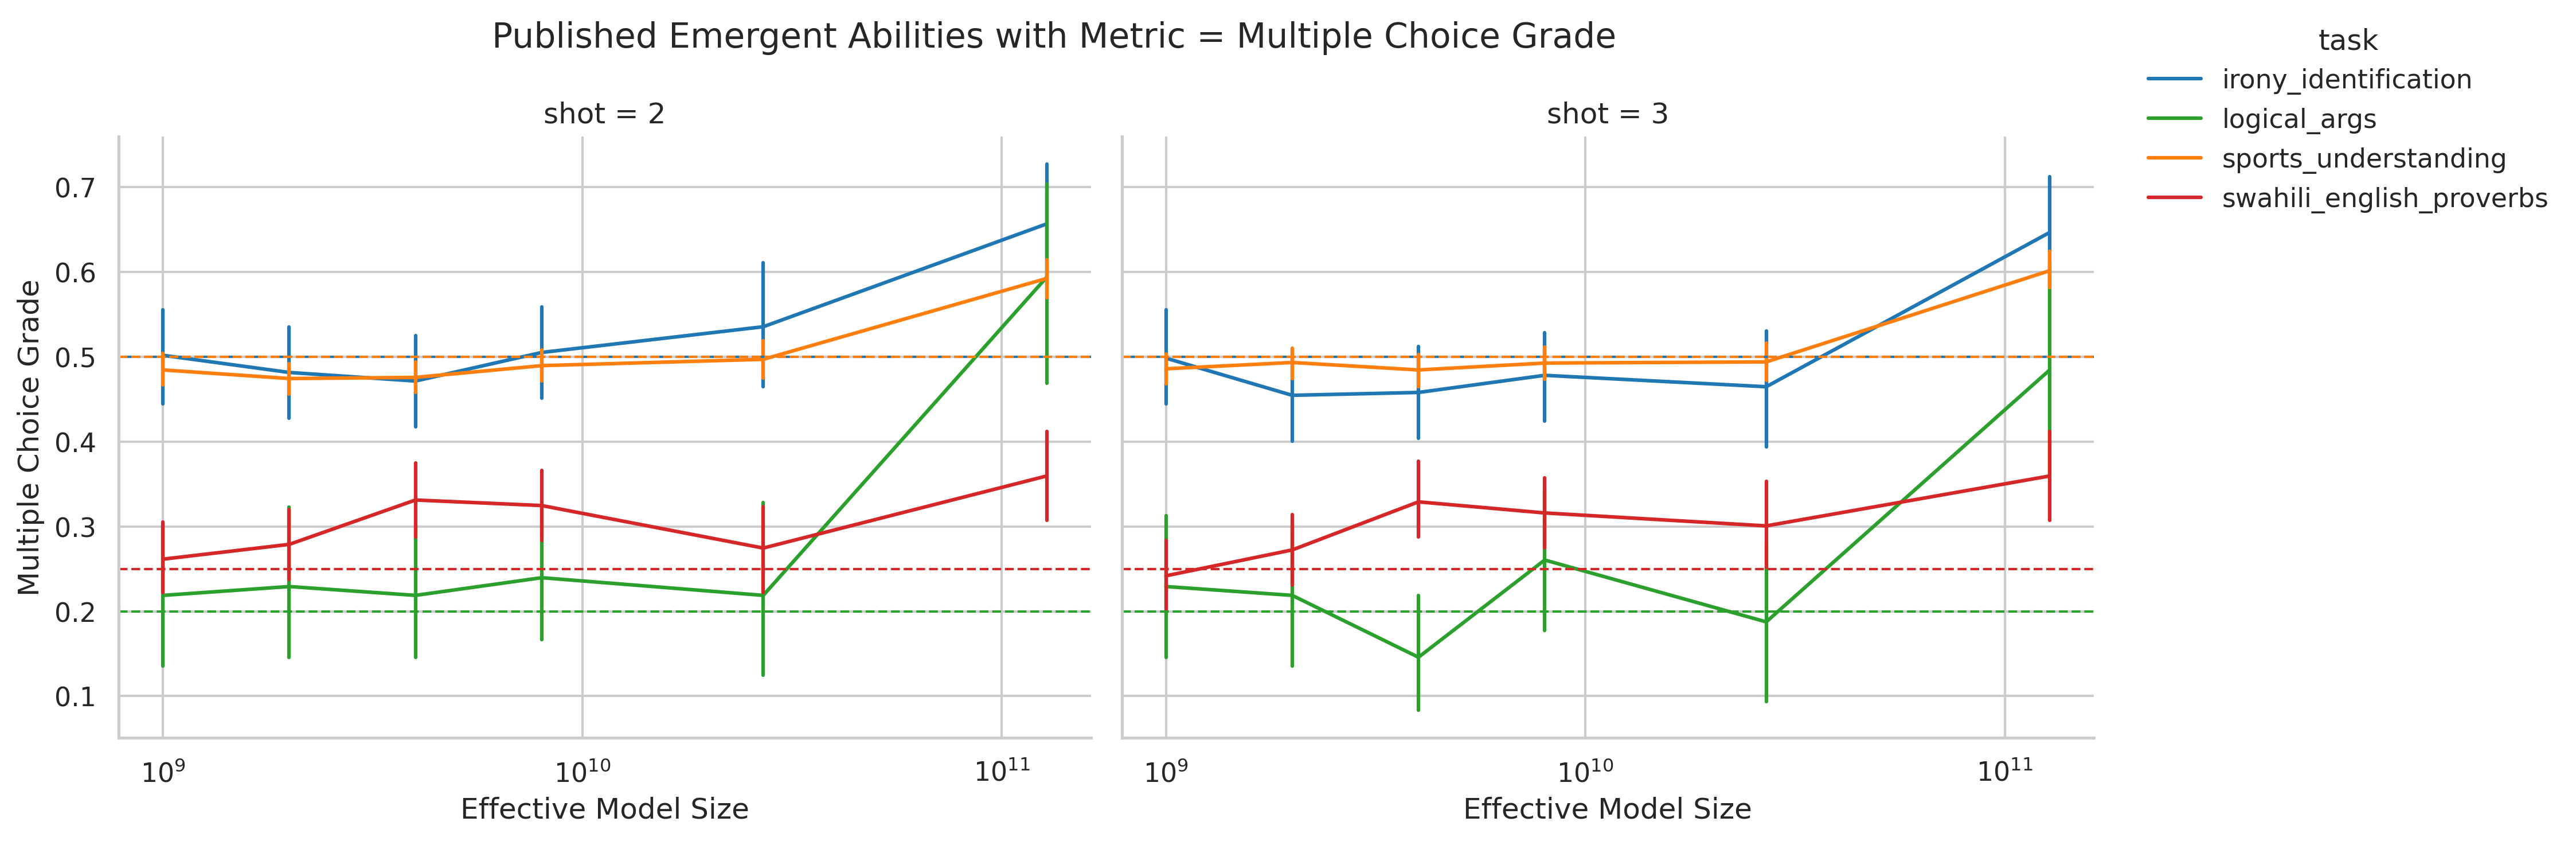
\includegraphics[width=0.49\textwidth]{figures/big_bench_emergent_tasks/score_vs_model_size_by_task_split_shot_other_metric=multiple_choice_grade.png}%
    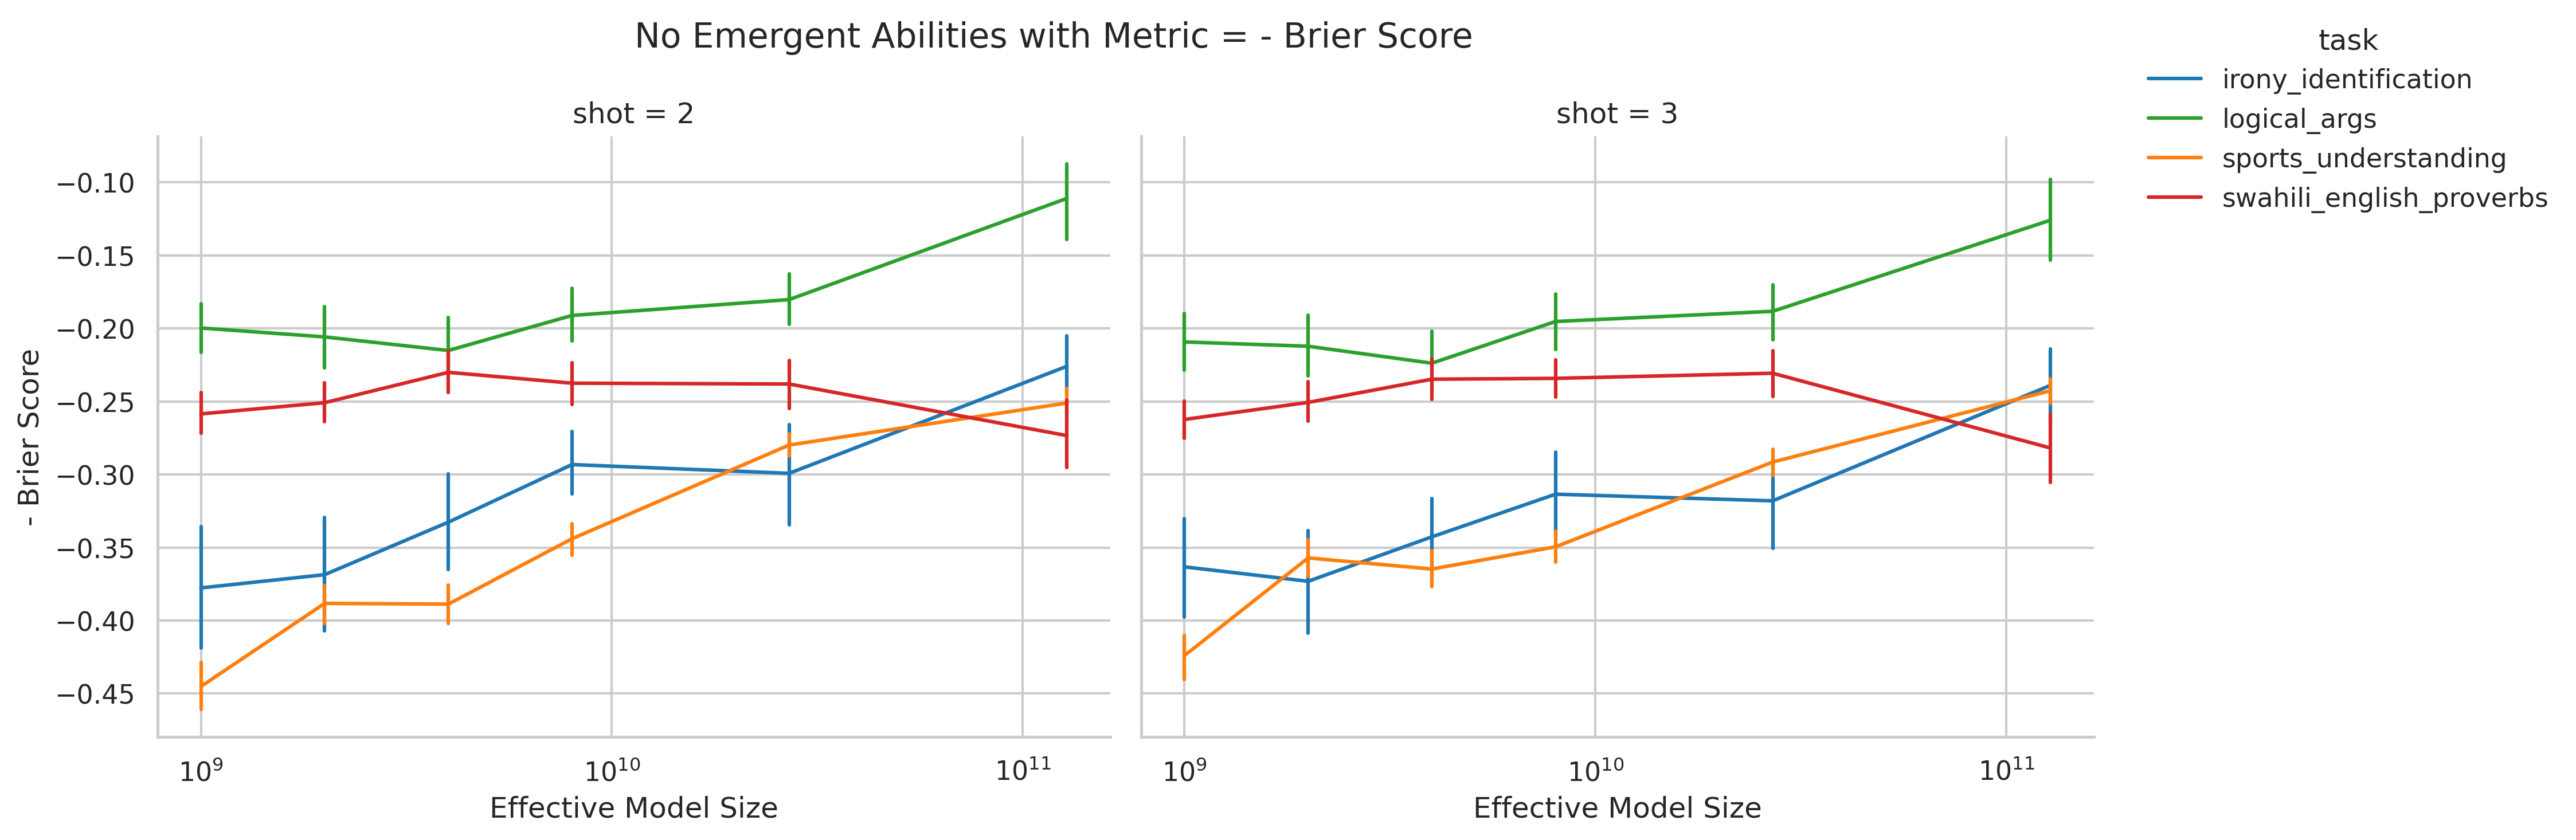
\includegraphics[width=0.49\textwidth]{figures/big_bench_emergent_tasks/score_vs_model_size_by_task_split_shot_other_metric=calibration_multiple_choice_brier_score.png}
    \caption{\textbf{Changing the metric when evaluating task-model family pairs causes emergent abilities to disappear.} Left: The LaMDA model family displays emergent abilities when measured under the discontinuous Multiple Choice Grade. Right: The LaMDA model family's emergent abilities disappear when measured under a continuous BIG-Bench metric: Brier Score.}
    \label{fig:big_bench_brier_score}
\end{figure}

\paragraph{Prediction: Changing Metric Removes Emergent Abilities}

% \footnote{BIG-Bench contains LaMDA models of sizes 16M, 53M, 125M, 244M, 422M.}
To test our second prediction, 
%we analyzed hand-annotated emergent abilities of \cite{wei2022bigbench}. 
we focused on the LaMDA family \cite{thoppilan2022lamda} because its outputs are available through BIG-Bench.
% whereas other model families' outputs are not.
%The smallest published LaMDA model has 2B parameters, but many LaMDA models in BIG-Bench are significantly smaller and we were unable to identify the sources of these smaller models, so we excluded them.
% according to \cite{wei2022bigbench}
For our analysis, we identified tasks on which LaMDA displays emergent abilities with Multiple Choice Grade, then asked whether LaMDA still displays emergent abilities on the same tasks with a different BIG-Bench metric: Brier Score \cite{brier1950verification}. 
Brier Score is a strictly proper scoring rule for predictions of mutually exclusive outcomes; for a binary outcome, the Brier Score simplifies to the mean squared error between the outcome and its predicted probability mass.
LaMDA's emergent abilities on the discontinuous Multiple Choice Grade disappeared when we changed the metric to the continuous Brier Score (Fig. \ref{fig:big_bench_brier_score}).
%This further supports our alternative explanation that emergent abilities are induced by the researcher's chosen metric.
These results support our alternative explanation that emergent abilities are induced by the chosen metric.
%, not unpredictable changes in the model family on a specific task with scale.